% Template for NIME 2017
%
% Modified by Cumhur Erkut on <2016-10-11 Tue>
% Modified by Edgar Berdahl on 5 November 2014
% Modified by Baptiste Caramiaux on 25 November 2013
% Modified by Kyogu Lee on 7 October 2012
% Modified by Georg Essl on 7 November 2011
%
% Based on "sig-alternate.tex" V1.9 April 2009
% This file should be compiled with "nime-alternate.cls"


\documentclass{nime-alternate}
\usepackage[utf8x]{inputenc}
\PrerenderUnicode{aâîțșĂÎÂȚȘ}
%\usepackage{dirtytalk}

\begin{document}
%
% --- Author Metadata here ---
\conferenceinfo{NIME'17,}{May 15-19, 2017, Aalborg University Copenhagen, Denmark.}

\title{SoundThimble: A High Resolution Gesture\\ Sonification Framework}

%
% You need the command \numberofauthors to handle the 'placement
% and alignment' of the authors beneath the title.
%
% For aesthetic reasons, we recommend 'three authors at a time'
% i.e. three 'name/affiliation blocks' be placed beneath the title.
%
% NOTE: You are NOT restricted in how many 'rows' of
% "name/affiliations" may appear. We just ask that you restrict
% the number of 'columns' to three.
%
% Because of the available 'opening page real-estate'
% we ask you to refrain from putting more than six authors
% (two rows with three columns) beneath the article title.
% More than six makes the first-page appear very cluttered indeed.
%
% Use the \alignauthor commands to handle the names
% and affiliations for an 'aesthetic maximum' of six authors.
% Add names, affiliations, addresses for
% the seventh etc. author(s) as the argument for the
% \additionalauthors command.
% These 'additional authors' will be output/set for you
% without further effort on your part as the last section in
% the body of your article BEFORE References or any Appendices.

\numberofauthors{4}
%
\author{
% You can go ahead and credit any number of authors here,
% e.g. one 'row of three' or two rows (consisting of one row of three
% and a second row of one, two or three).
%
% The command \alignauthor (no curly braces needed) should
% precede each author name, affiliation/snail-mail address and
% e-mail address. Additionally, tag each line of
% affiliation/address with \affaddr, and tag the
% e-mail address with \email.
%
% 1st. author
\alignauthor
Ben Trovato\\
       \affaddr{Authors hidden for review}\\
       \affaddr{1932 Wallamaloo Lane}\\
       \affaddr{Wallamaloo, New Zealand}\\
       \email{trovato@corporation.com}
% 2nd. author
\alignauthor
G.K.M. Tobin\\
       \affaddr{Authors hidden for review}\\
       \affaddr{P.O. Box 1212}\\
       \affaddr{Dublin, Ohio 43017-6221}\\
       \email{webmaster@marysville-ohio.com}
%\and
% 3rd. author
%\alignauthor Grigore Burloiu\\
%       \affaddr{CINETic}\\
%       \affaddr{UNATC "I.L. Caragiale"}\\
%       \affaddr{Bucharest, Romania}\\
%       \email{gburloiu@gmail.com}
% 4th. author
%\alignauthor Bogdan Golumbeanu\\
%\affaddr{CINETic}\\
%\affaddr{UNATC "I.L. Caragiale"}\\
%\affaddr{Bucharest, Romania}\\
%\email{bogdangolumbeanu@yahoo.com}
}
% There's nothing stopping you putting the seventh, eighth, etc.
% author on the opening page (as the 'third row') but we ask,
% for aesthetic reasons that you place these 'additional authors'
% in the \additional authors block, viz.
%\additionalauthors{Additional authors: John Smith (The Th{\o}rv{\"a}ld Group,
%email: {\texttt{jsmith@affiliation.org}}) and Julius P.~Kumquat
%(K. Consortium, email: {\texttt{jpkumquat@consortium.net}}).}
\date{24 Jan 2017}
% Just remember to make sure that the TOTAL number of authors
% is the number that will appear on the first page PLUS the
% number that will appear in the \additionalauthors section.

\maketitle
\begin{abstract}
	
	
%\textit{SoundThimble} is an interactive installation, inspired by the game called Hunt the Thimble in which someone hides an object then guides the other players to its location by stating whether their position is “hot” – closer to the object, or “cold” – farther from the object. 


 The installation is based on a state-of-the-art Vicon motion capture system, used alongside a Max-based platform to track, interpret and sonify the movement and gestures of a performer in 3D space.
\end{abstract}

\keywords{sonification, motion tracking, gesture spotting, interactive installation, synthesis}

\acmclassification1998{
\begin{itemize}
	\setlength\itemsep{-0.2em}
	\item Applied computing~$\rightarrow$~Sound and music computing
	\item Computing methodologies~$\rightarrow$~Motion capture
	\item Human-centered computing~$\rightarrow$~Gestural input
	\item Human-centered computing~$\rightarrow$~Auditory feedback
\end{itemize}

}

 
% \ccsdesc[500]{Computing methodologies~Motion capture}
% \ccsdesc[500]{Applied computing~Sound and music computing}
% \ccsdesc[300]{Human-centered computing~Auditory feedback}
% \ccsdesc[300]{Human-centered computing~Gestural input}

\section{Introduction}

%- motivation

%- challenges

%\textbf{- the Vicon system}\\ \par


High resolution three-dimensional motion capture systems are traditionally used for animation in film and games~\cite{animatie}, as well as for life sciences research~\cite{life} and engineering applications~\cite{eng}. This technology has long been mined by the NIME community~\cite{dobrian2003gestural, nymoen2011soundsaber}, although in many early cases, technological limitations meant that the motion data transmission and the sound generation processes were not simultaneous~\cite{dobrian2003gestural, kapur2005framework}.


The \textit{SoundThimble} project harnesses current motion tracking technology and gesture detection algorithms to develop new modes of sound exploration in an interactive installation context. Our aim is to push beyond the standard paradigms of isolated body motion audification~\cite{dobrian2003gestural,kapur2005framework} or parameter mapping-based new instruments~\cite{nymoen2011soundsaber}, towards deeper narrative structures coupled with layered arrangement of music patterns.


Our implementation uses a state-of-the-art Vicon motion capture system\footnote{See  \url{https://www.vicon.com}.} based on eight Vantage 5-megapixel infrared cameras and two Bonita video cameras. Since the open-source software developed in this project\footnote{Available at  \url{https://github.com/RVirmoors/viconOSC}.} is\linebreak built around Vicon's Datastream SDK,\footnote{See  \url{https://www.vicon.com/products/software/datastream-sdk}.} the platform can be ported to both older and future Vicon-based systems.

In the remainder of the paper, we review relevant existing projects and technology (section~\ref{sec:related}), we describe the \textit{SoundThimble} concept and development (section~\ref{sec:proj}), we analyse two practical case studies (section~\ref{sec:case}), and we conclude with a survey of remaining challenges and future perspectives (section~\ref{sec:conc}).


\section{Related Work}
\label{sec:related}


- interactive / movement sonification examples\cite{hermann2011sonification}.

- Vicon \& related projects



10+ year history of Vicon+sonification



- micro

\cite{worrall2013understanding}


- vicon + OSC de la iem.at

The current decade has seen qualitative advances in the interaction between human gesture and sound behaviour~\cite{Gestureanalysis}. ... \cite{probabilisticmodels}.

\section{Project Description}
\label{sec:proj}

\subsection{Concept}

% inovare = abordarea spatializarii obiectelor sonore / acusmatics

The sound-thimble, as the basic building block of our framework, is based on the concept of \textit{sound object} in the Schaefferian sense, as a clearly delimited sounding unit, open to manipulation, arrangement and composition~\cite{schaeffer1998solfege}.

Such an entity, once instanced, can retain an ambiguous nature (spatially and acousmatically) or can switch to a more material state (positioned in space and tied to a causal source)~\cite{soundunseen}. The duality between the latent positioning of the object (which can be inferred from phenomena other than spatial sound reproduction), and the active sound spatialisation, once tied to motion data, becomes an innovative tool for sonic arts through sound sketching, auditory games and other realtime interaction scenarios.

\subsubsection{Interaction scenario}

\textit{SoundThimble} can be viewed as both an interactive sound installation and an auditory game, comprising three phases: search, manipulation, arrangement.


The game's narrative starts with a human player attempting to find a sound-thimble (a stationary virtual object, randomly positioned in 3D space), by analysing cues that are constantly shifting in the sonic fabric based on the human's movement relative to the object. Analogously to the traditional game of \textit{Hunt the Thimble} (a.k.a \textit{Hot or Cold}), the space between the human and the virtual object is correlated to sound synthesis and modulation parameters. Briefly, the closer one comes to the object, the more coherent the sound and vice-versa. 

Once the object is found, its sonic manifestation gains a richer causal relationship to the human: the player becomes a performer, and is now able to explore the object's sonic palette, and record a number of gestures that can be re-performed later, re-called, and used to trigger or manipulate sonic shifts and events.

Finally, the performer can drop the virtual object to the floor, or discard it by ``pushing" it outside of the installation boundaries. This triggers a new object to be randomly generated, while the player retains a degree of control over the initial object via the recorded gestures. Both objects are now in a latent state, with the new one guiding the player's search, and the previous one responding to the learned set of gestures.

This repeating scenario is outlined in Figure~\ref{fig:concept}: objects are randomly generated, the performer finds them, defines gestures and interacts sonically with them before arranging them in a pleasing configuration. With each spawning of a new object or assignment of a new gesture, the game becomes more challenging and complex, but also more flexible and rewarding.


\begin{figure}[t]
	\centering
	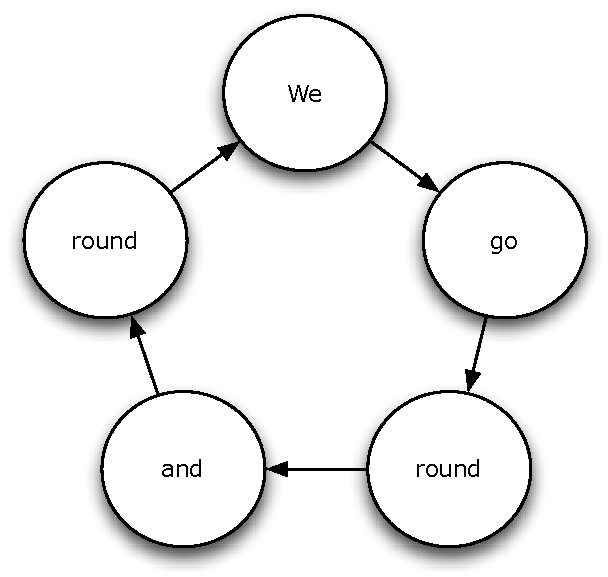
\includegraphics[width=1\columnwidth]{img/BlockDiagram1}
	\caption{... diagram}
	\label{fig:concept}
\end{figure}

\subsubsection{Performance aesthetic}

- text Bogdan

\subsection{Implementation}

=== FIG: Framework Diagram: Camere, Nexus, C++, Max, Speakers ====


%Many interactions and programable elements which are included in the concept have an exactly function and usefulness. These elements are created in MAX with the help of Vicon SDK and OSC C++ library. The concept suppose an interactive action of a performer or a simple user with an virtual object which has associated gestures defined by person. Virtual object interaction acts in sound design utility like a master controller. Searching for a certain object comes with an audio feedback which makes the search easier. Object's asscociated gestures are compatible with sound design patch and contribute at audio performance. A dynamic mapping of marker's coordinates is necessary to transfer data between Nexus and MAX.

One of the first challenges was to create a method of sending real-time from Vicon to MaxMSP where data would be processed and used to generate and manipulate sound. By default, the Vicon system does not support the Open Sound Control (OSC) protocol (ref), needed to communicate with MaxMSP. To overcome this limitation, some code modifications and additions have been implemented inside Vicon’s Blade sdk.



\subsubsection{Character design}

Figure~\ref{fig:nexus} shows the Vicon Nexus software 

=== FIGURE : Nexus / Bogdan ====



Implementation of the concept presented above requires Nexus, Vicon SDK and MAX sotware. Every character involved in the scene is defined by a limited number of markers. In this case, two markers are positioned on the head, one marker is positioned on elbow and the others 2 on the hand (thumb and index finger). Every marker has associated a name in Nexus and between them 6 segments are drawn. It is very important in realtime capture motion, that the marker to have assigned correct coordinates.

- \textbf{Vicon extensions (SDK plugin)} \par
Vicon's SDK is a versatile and simple tool for users to gain easy access to Vicon DataFlow created in Nexus, Blade or Tracker applications.The Vicon DataStream Software Development Kit (SDK) provides intuitive programable access to data with custom functions created in C++. With the help of some functions, Vicon's SDK forwardes the Vicon DataStream to other constructive softwares and plug-ins to create custom applications \footnote{See \url{https://www.vicon.com/products/software/datastream-sdk/}.}. In combination with Open Sound Control protocol, Vicon's SDK forwards data to any software compatible with this communication protocol (eg. MAX). OSC is a protocol for communication among computers, sound synthesizers and other multimedia devices\footnote{See  \url{http://opensoundcontrol.org}.}. Hence, any marker can be routed in MAX using its parameters and coordinates. Also, the Vicon DataStream Software Development Kit (SDK) admits inside changes such as labeling markers, timecode generation and framerate.

\subsubsection{Object generation \& interaction mechanics}
%GRIG: nu e cazul sa prezentam Max pe larg aici. Eventual o propozitie scurta mai sus...
%Max is a realtime visual programing environment for music and multimedia arts that helps you build stand-alone applications, plugins and mixing audio signals. In order to create interactive sounds, attractive grapichs and special effects, MAX creates a connection between virtual objects and subpatches\footnote{See \url{http://www.cycling74.com/}.}.
Manipulating objects algorithm consists of some big steps: object generation, finding the object, picking up the object, throwing the object on the floor. 
%GRIG: ar mai fi picking up the object, si eventual throwing...

Object generation is realized by random generators with the help of \textit{drunk} object, but with certain limits. These limitations are influenced by the dimensions of the room in which the Vicon system is installed. Finding the object supposes continuous mathematic operations between the coordinates of the object and coordinates of the left hand's marker. This process comes with an audio feedback. When these coordinates are close enough one to another, the object is retreived and manipulated by performer (eg. define gesture). After all these processes, a simple comparison between the coordinates of the floor and the value of the z axes of the marker is done in order to put down the object. According to this, a performer can handle as many objects as he wants.\\ \par


\subsubsection{Gesture recognition}

 \textit{Mubu} containers provided by Ircam laboratories in MAX software represent a handy tool to record and analyze gesture, captured with Vicon system \cite{mubu}. Our gesture recognition algorithm is based on Hierarchical Hidden Markov Models (HHMM) implemented in \textit{mubu.hhmm} object of MAX/MSP. HHMMs are a generalization of HMM where each state is considered to be a self-contained probabilistic model \cite{hhmm}. The system is trained by captured data which is essentially a gesture. This process requires a predefined indicator in order to delimitate gestures from all data flow. The algorithm analyzes all input data and generates a probability of similarity between data and saved gestures. In order to control every generated object, there are associated 2 or 3 gestures saved by the performer, but there is a limited time for the gestures to be executed. Predefined gestures offer the possibility to delete the gesture just saved and also indicate the moment the gesture is recorded.

\subsubsection{Sound design}

Although there is a wide range of sonification alternatives available, including triggering of pre-stored sounds, modulating/LFO-ing stored sounds etc. we started experimenting with a few synthesis patches with parameters that could be correlated to XYZ coordinates in a reactive and expressive manner.  In order to exploit the increased spatial resolution, marker positions, grouping of markers and other possibilities of the Vicon system, the development of synthesis  algorithms in MaxMSP seems to be very flexible.  In this way, the whole soundscape can be generated in a continuous, organic manner by correlating markers’ positions with synthesis parameters. 

The interactive experience can be described as having two main paradigms: object finding and object interaction. For object finding we have been experimenting with two straightforward patches in MaxMSP: the first is based on a sawtooth wave that is sent to 8 delays. These output a random signal with a settable range which continuously alter the phase and frequency of the sawtooth iterations. This chorus-inspired algorithm has three controllable parameters: main frequency, range and speed of frequency variation. The farthest someone is from the virtual object the more detuning and phase shifting occurs on each of the eight iterations, while approaching it the effect becomes less pronounced to the point where only slight variations of the signal occur. Also, main frequency is associated with movement in the vertical plane. Further modulation can be used to make the sound more complex. The second patch is somewhat based on the same principle of decorrelation: six sine waves with different frequencies are modulated in amplitude by a random~ object which generates control waves with a variable degree of complexity (more or less noise-like shapes). As in this case, distance between the performer and the virtual object is associated with the level of randomness and decorrelation: longer distance translates to a higher degree of decorrelation and randomness. What is interesting about this patch is the effect of amplitude modulation (AM) (referinta ce e AM) when the carrier frequency (?) goes beyond 20hz and sidebands occur. By using noise-like carriers, complex sonorities occur with a variable harmonic content. In both cases, the performer tries to find the object by listening to these variations. By correlating small and large variations to its position in the 3d field the performer receives meaningful clues about where the object might be as well as an interesting and engaging soundscape. 

An additional granular synthesis (ref) patch that was initially created for object interaction also seems to be effective for object finding. The patch reads short grains from a pre-loaded sound and scatters into “clouds” in either a controlled or random manner. Among the parameters that can be mapped are: grain position, grain size, envelope shape, level of scattering, pitch, stereo width. Not only this, but by using the [pattrstorage] and [pattr] objects we can group multiple parameters’ state, save them as presets and interpolate between them. By doing this, we can control an undefined number of parameters by linking only one marker/one gesture to the interpolation amount box. This patch also seems to be effective for finding the object, differentiating the two paradigms by the level of control: less control for object finding and more control for object interaction.

Real-scenario testing and simulations using the Vicon cameras is quite limited because two main reasons: we don’t always have access to the space and we would always need a performer that could cope with long hours of code debugging, errors, MaxMSP programming and so on. This is the reason why in order to simulate interactions inside the sound design patches, we also created a basic interface in Jitter that receives data from Vicon Blade via OSC and represents each marker in the 3d space. By using this interface it is possible to move a particular marker anywhere along the XYZ planes, by only using the mouse, and get instant auditory feedback. The downside being that experiments done in virtual space do not always translate well to the real space: calibration by value scaling, experimenting with different function shapes etc. is tedious but absolutely necessary.

So far, all sound-design is based on two channels that can either be routed to multiple pairs of speakers or downmixed to mono and diffused on an arbitrary number of speakers, however multichannel sound is taken into consideration for future improvements.


- Visualisation (jitter)

\section{Case studies}
\label{sec:case}


\subsection{Interactive Installation}

- performance analysis

\subsection{Performance}



\section{Conclusions and Future Work}
\label{sec:conc}
- Areas of improvement

- Eye tracking?

%Although we have been working on the project for only a few months it is fairly safe to state that the expressive opportunities of the Vicon system are superior to others such as cameras and Microsoft Kinects. Although a lot more challenging (no native OSC support, difficulties in conducting test at any time, arduous task of integrating Blade to the Jitter interface to the Gesture Recognition patch, and then to the Sound Synthesis patch, great deal of calibration and scaling), new other possibilities are being offered by the high temporal and spatial resolution.

Future work on SoundThimble could/will include: multiple performers, eye tracking, generative visuals, spatial sound, more powerful synthesis and sound manipulation algorithms, different rules added to the narrative of the auditory game.


%ACKNOWLEDGMENTS are optional
\section{Acknowledgments}
%Our project is hosted by the CINETic research centre.\footnote{See \url{https://cinetic.arts.ro}} We wish to thank Ștefan Pârlog for video production and additional research, Mihai Gheorghiu for additional sound design, and Vlad Constantin for additional research.
Hidden for review.

%
% The following two commands are all you need in the
% initial runs of your .tex file to
% produce the bibliography for the citations in your paper.
\bibliographystyle{abbrv}
\bibliography{sonif-ref} 
\textbf{TO DO}: review bib!

% That's all folks!
\end{document}
